\section{Theory}

\subsection{The Cost Function }
\label{sec:cost_fn}

\label{sec:theory}

** the model in (ADL, 1993),
we consider a cost function of the form

\begin{equation}
  \label{eq:cost-t_d}
  C(t_d; \alpha, \beta, \gamma, t^*) = \alpha tt(t_d) + \beta[t^*-t_d-tt(t_d)]^+ + \gamma[t_d+tt(t_d)-t^*]^+ 
\end{equation}
where
\begin{itemize}
\item \(t_d\) is a possible departure time, on which the cost depends
\item \(t^*\) is the desired arrival time
\item \(\alpha\) is the value of time spent travelling
\item \(\beta\) is the value of time spent waiting there
\item \(\gamma\) is the value of time arriving late
\item \(tt(t_d)\) is the time spent travelling if leaving at time \(t_d\)
\item \([x]^+ = \max(0, x)\)
\end{itemize}

We will consider, in this article,
how the cost depends on the time at which a person arrives,
rather than the time at which the person departs.
Since the travel time is known without uncertainty,
the users will then be able to make a choice based on their arrival time.

Let thus
\begin{equation}
  \label{eq:t_a-t_d}
  t_a(t_d) = t_d + tt(t_d)
\end{equation}
be the function linking the departure time to the arrival time.
The following holds:
\begin{obs}
  The function \(t_a(t_d)\) is invertible
\end{obs}
This simply follows from noting that  \(t_a(t_d)\) must be strictly increasing:
this corresponds to the traffic following a First In First Out (FIFO) logic,
that is, a later departure cannot result in an earlier arrival:
a reasonable assumption that we make on the travel time function\footnote{Note that this assumption is equivalent to assuming the decrease of the travel time function to be bounded: computing the derivative of the function \(t_a\), we find that it being increasing is equivalent to \(tt'(t_d) > -1\ \forall\. t_d\)}.

The function \(t_d(t_a)\) that, given an arrival time,
yields the unique departure time that would result in the given arrival,
is thus well defined.
The travel time function can thus be defined in term of the arrival time:
\begin{definition}
  \label{def:tta}
  Let
  \begin{equation*}
    tt:\R \rightarrow \R
  \end{equation*}
  be a function expressing the travel time in terms of the departure time.
  The function \(tt_a\), expressing the travel time in terms of the arrival time, is defined as follows:
  \begin{equation*}
    tt_a(t_a) = tt(t_d(t_a))
  \end{equation*}
\end{definition}

By using equation \eqref{eq:t_a-t_d} and Definition~\ref{def:tta}, the expression for the cost in~\eqref{eq:cost-t_d} simplifies,
trivially becoming

\begin{equation}
  \label{eq:cost-t_a}
  C(t_a; \alpha, \beta, \gamma, t^*) = \alpha tt_a(t_a) + \beta[t^*- t_a]^+ + \gamma[t_a - t^*]^+ 
\end{equation}
where the dependency of \(t_a\) on the departure time \(t_d\) has been hidden:
the arrival time can indeed be directly observed,
and its dependency on the departure time neglected.

In the following article,
the expression used will be the one given the arrival time, as shown in~\eqref{eq:cost-t_a},
being that a simpler expression if compared to the original one in~\eqref{eq:cost-t_d}.

We will, lastly normalize \(\alpha\) to 1.
This is possible since the cost can be considered up to a multiplicative constant.
Instead of the real cost \(C\) we will thus consider a scaled version of it \(C/\alpha\),
and minimize the following:
\begin{equation}
  \label{eq:cost_final}
  C(t_a; \beta, \gamma, t^*) = tt_a(t_a) + \beta[t^*- t_a]^+ + \gamma[t_a - t^*]^+ 
\end{equation}

The notation is here ambiguous regarding the cost \(C\) and the coefficients \(\beta,\gamma\).
It anyway doesn't lose in generality, and was chosen for simplicity.

\subsection{Minimum of the Cost Function}
\label{sec:cost_minima}

Consider hence the cost in \eqref{eq:cost_final},
and the problem of finding the minimum of it.
Before computing the first order condition,
in order to find the global minimum it is useful to do some qualitative reasoning on the values taken by the cost function.

Note that, indeed, a value \(t_0\) for the arrival time can only be greater,
smaller or equal to the given \(t^*\).
In the following definition,
the two cases are separated, so that they can be studied independently.
\begin{definition}
  Let values for the parameters \(\beta, \gamma, t^*\) be fixed.
  \begin{itemize}
  \item The \textit{optimal early arrival} \(t_e^{opt}\) is the early arrival realizing the least cost:
    \begin{equation*}
      t_e^{opt}(\beta, \gamma ,t^*) = \argmin_{t_a < t^*}C(t_a; \beta, \gamma, t^*)
    \end{equation*}
  \item The \textit{optimal late arrival} \(t_l^{opt}\) is the late arrival realizing the least cost:
    \begin{equation*}
      t_l^{opt}(\beta, \gamma ,t^*) = \argmin_{t_a > t^*}C(t_a; \beta, \gamma, t^*)
    \end{equation*}
  \item The \textit{optimal arrival} \(t^{opt}\) is the arrival realizing the least cost:
    \begin{equation*}
      t^{opt}(\beta, \gamma ,t^*) = \argmin_{t_a}C(t_a; \beta, \gamma, t^*)
    \end{equation*}
  \end{itemize}
\end{definition}

Please note that in general,
optimal early and late arrivals may not exist,
depending on the choice of the travel time function and the parameters.

For studying where these minima occur, consider now the case of an early arrival \(t_a = t_0 < t^*\).
Since
\begin{equation*}
  t_0 - t^* < 0
\end{equation*}
the cost simplifies, becoming
\begin{align}
  C(t_0; \beta, \gamma, t^*) & = tt_a(t_0) + \beta[t^*- t_0]^+ + \gamma[t_0 - t^*]^+ \nonumber \\
                             & = tt_a(t_0) + \beta(t^*- t_0)\label{eq:cost_early}
\end{align}

\begin{figure}
  \centering
  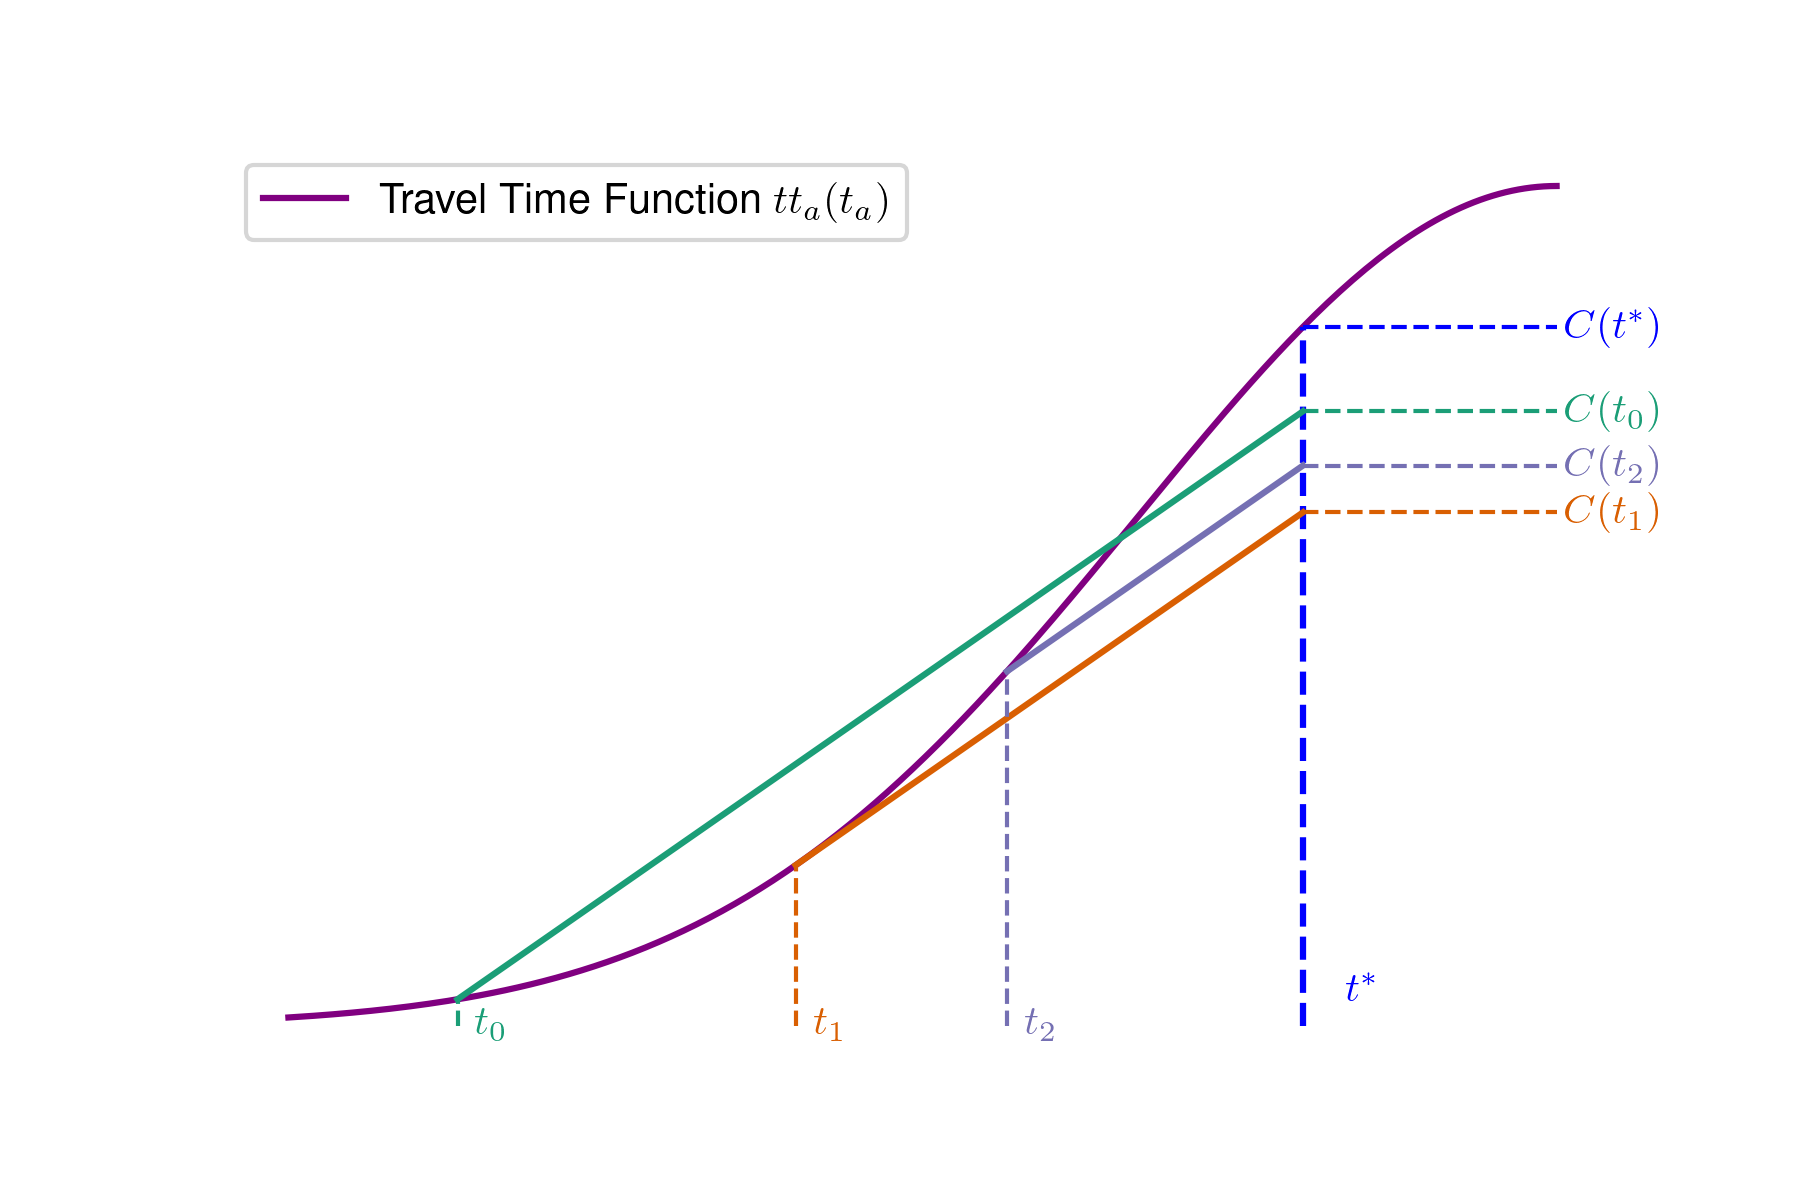
\includegraphics[width=.8\textwidth]{early_arrivals_cost}
  \caption{Dependency of the cost on the arrival time.
    The solid lines are parallel, of slope \(\beta\).
  Note that their distance is thus the only factor affecting the cost of an early arrival}
  \label{fig:early_arrivals_cost}
\end{figure}

The cost will thus be, as expected,
the sum of the travel time and a term linear on the distance of the actual arrival from the desired one.

Figure \ref{fig:early_arrivals_cost} displays how the cost of an early arrival changes when varying the arrival time:
the cost is only determined by the distance of the lines of slope \(\beta\) between each other, that is,
the projected distance of the points \(tt_a(t_a)\) on the axis orthogonal to the lines determining the cost
(the one described by \(y = -x/\beta\)).

This reasoning leads to the following lemma:
\begin{lemma}
  \label{lemma:cost_decoupled}
  If an optimal early arrival \(t_e^{opt}\) exists,
  it can be found by solving a simple minimization problem:
  \begin{equation*}
    t_e^{opt} = \argmin_{t_a < t^*} tt_a(t_a) - \beta t_a
  \end{equation*}

  Similarly, if an optimal late arrival exists,
  it is
  \begin{equation*}
    t_l^{opt} = \argmin_{t_a > t^*} tt_a(t_a) + \gamma t_a
  \end{equation*}
\end{lemma}
\begin{proof}
  The claim for early arrivals simply follows from the expression for the cost in~\eqref{eq:cost_early}:
  the following indeed holds for \(t_a < t^*\)
  \begin{align*}
    C(t_a; \beta, \gamma, t^*) & = tt_a(t_a) + \beta(t^*- t_a) \\
                               & = tt_a(t_a) + \beta t^* - \beta t_a
  \end{align*}

  But \(\beta t^*\) is clearly constant in \(t_a\),
  and minimization is invariant on translations.
  This yields
  \begin{align*}
    t_e^{opt} & = \argmin_{t_a < t^*} C(t_a) \\
              & = \argmin_{t_a < t^*} tt_a(t_a) + \beta t^* - \beta t_a \\
              & = \argmin_{t_a < t^*} tt_a(t_a) - \beta t_a
  \end{align*}

  Regarding late arrivals, the argument is symmetrical and thus omitted.
\end{proof}

Note that this has some trivial implication on the value of the derivative of the travel time function at the optimal points:
\begin{obs}
  The derivative of the travel time function \(tt_a'\) is fixed in the optimal points:
  \begin{itemize}
  \item \(tt_a'(t_e^{opt}) = \beta\)
  \item \(tt_a'(t_l^{opt}) = -\gamma\)
  \end{itemize}
\end{obs}

This follows from the Lemma above:
if the function \(tt_a\) is differentiable, being the minima computed over an open set,
if they exist they necessarily satisfy the first order conditions:
for the early arrivals, they are
\begin{align*}
  \diffp{}{{t_a}} \left(tt_a(t_a) - \beta t_a\right) & = 0 \\
  tt_a'(t_a) & = \beta
\end{align*}

The case for late arrival is analogous.

While not particularly difficult to retrieve,
the expression in Lemma~\ref{lemma:cost_decoupled} is useful,
since it makes a clearer decoupling of the dependencies of the point that minimizes the cost on the parameters \(\beta, \gamma\) and \(t^*\).
We can indeed see how changing the parameters affects the 

%%% Local Variables:
%%% mode: LaTeX
%%% TeX-master: "../main"
%%% End:
